\chapter{Laufzeitsicht}

\newcommand{\commentTwo}[1]{}

\commentTwo{
	@startuml
	title Laufzeitsicht 2: Asynchroner RPC-Anfragedurchlauf inkl. Namensauflösung
	
	participant "Client\nApplikation" as ClientApp
	participant "Client-Proxy\n(Stub)" as ClientProxy
	participant "Naming Service" as NamingService
	participant "Marshalling" as Marshalling
	participant "Async RPC Sender" as RPCSender
	participant "Message Transport\n(z.B. TCP)" as Transport
	participant "Async RPC Receiver" as RPCReceiver
	participant "Unmarshalling" as Unmarshalling
	participant "Server-Skeleton\n(Stub)" as ServerSkeleton
	participant "Server\nApplikation/\nNode Logik" as ServerApp
	
	ClientApp -> ClientProxy : RPC-Aufruf(Dienstname, Argumente)
	activate ClientProxy
	' Der Client-Proxy agiert als Stellvertreter [12, 13] und benötigt die Adresse für den Dienst [6, 7]
	ClientProxy -> NamingService : **auflösen**(Dienstname)
	activate NamingService
	' Der Naming Service löst den logischen Dienstnamen in eine Netzwerkadresse auf [6-11]
	NamingService --> ClientProxy : Dienstadresse
	deactivate NamingService
	
	ClientProxy -> Marshalling : **serialisiere**(Argumente)
	activate Marshalling
	' Argumente werden serialisiert [6-8]
	Marshalling --> ClientProxy : serialisierte_Argumente
	deactivate Marshalling
	
	ClientProxy -> RPCSender : **sende_Anfrage**(serialisierte_Argumente, Dienstadresse)
	deactivate ClientProxy
	activate RPCSender
	' Anfrage wird über den Sender verschickt [4, 6]
	RPCSender -> Transport : sende_Nachricht(Request-Paket)
	activate Transport
	deactivate RPCSender
	' Nachrichtentransport [allgemeines Konzept]
	
	Transport -> RPCReceiver : **liefere_Nachricht**(Request-Paket)
	deactivate Transport
	activate RPCReceiver
	' Nachricht empfangen
	RPCReceiver -> Unmarshalling : **deserialisiere**(Request-Daten)
	activate Unmarshalling
	' Daten werden deserialisiert [6-8]
	Unmarshalling --> RPCReceiver : deserialisierte_Daten
	deactivate Unmarshalling
	
	RPCReceiver -> ServerSkeleton : Methodenaufruf(deserialisierte_Daten)
	deactivate RPCReceiver
	activate ServerSkeleton
	' Server-Skeleton ruft Methode auf [12, 13]
	ServerSkeleton -> ServerApp : **rufe_Methode_auf**(Argumente)
	activate ServerApp
	' Server-Logik wird ausgeführt
	' Bei asynchronem RPC läuft die Antwortverarbeitung oder ein Callback separat.
	...
	ServerApp --> ServerSkeleton : (Verarbeitung läuft asynchron im Hintergrund)
	deactivate ServerApp
	ServerSkeleton --> RPCReceiver : (keine synchrone Antwort auf diesem Request-Pfad erwartet)
	deactivate ServerSkeleton
	@enduml	
}



\section{Szenario U1}
\textbf{Information Weiterleiten}\\
\begin{figure}[h!]
    \centering
    \includegraphics[width=0.8\linewidth]{diagrams/Information_Weiterleiten.png}
    \caption{Information Weiterleiten}
    \label{fig:Information_Weiterleiten}
\end{figure}


\section{Szenario U2}
\textbf{Node Registrieren}\\
\begin{figure}[h!]
    \centering
    \includegraphics[width=0.8\linewidth]{diagrams/Node_Registrieren.png}
    \caption{Node Registrieren}
    \label{fig:Node_Registrieren}
\end{figure}

\section{Szenario U3}
\textbf{Namensauflösung}\\
\begin{figure}[h!]
    \centering
    \includegraphics[width=0.8\linewidth]{diagrams/Namen_auflösen.png}
    \caption{Namensauflösung}
    \label{fig:Namensauflösung}
\end{figure}


\section{Szenario U4}
\textbf{Marshalling}\\
\begin{figure}[h!]
    \centering
    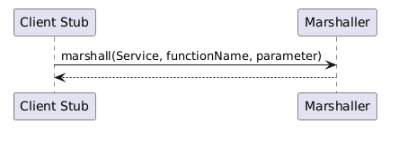
\includegraphics[width=0.8\linewidth]{diagrams/Marshalling.png}
    \caption{Marshalling}
    \label{fig:Marshalling}
\end{figure}

\section{Szenario U5}
\textbf{Transport}\\
\begin{figure}[h!]
	\centering
	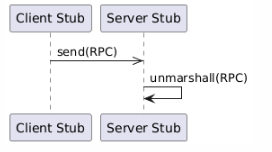
\includegraphics[width=0.8\linewidth]{diagrams/Transport.png}
	\caption{Transport}
	\label{fig:Transport}
\end{figure}


\section{Szenario U6}
\textbf{Sicherheit}\\
\begin{figure}[h!]
	\centering
	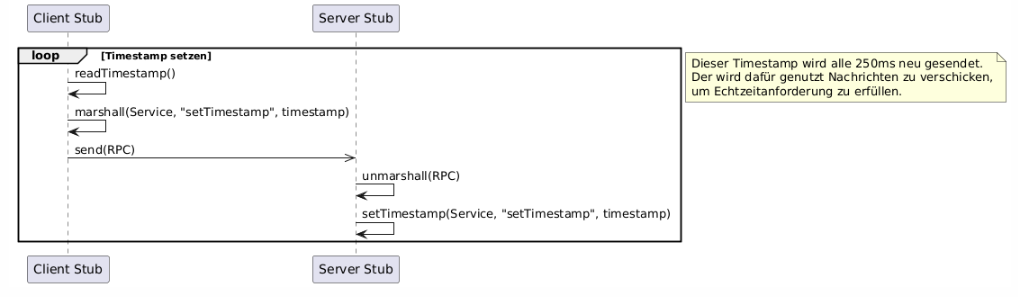
\includegraphics[width=0.8\linewidth]{diagrams/Sicherheit.png}
	\caption{Sicherheit}
	\label{fig:Sicherheit}
\end{figure}


%TODO need a runtimeview for Fehlertransparenz
% \section{Szenario U7}
% \textbf{Fehlertransparenz}\\
% \begin{figure}[h]
% 	\centering
% 	\includegraphics[width=0.8\linewidth]{diagrams/Fehlertransparenz.png}
% 	\caption{Fehlertransparenz}
% 	\label{fig:Fehlertransparenz}
% \end{figure}

\section{Szenario U8}
\textbf{Watchdog}\\
\begin{figure}[h!]
	\centering
	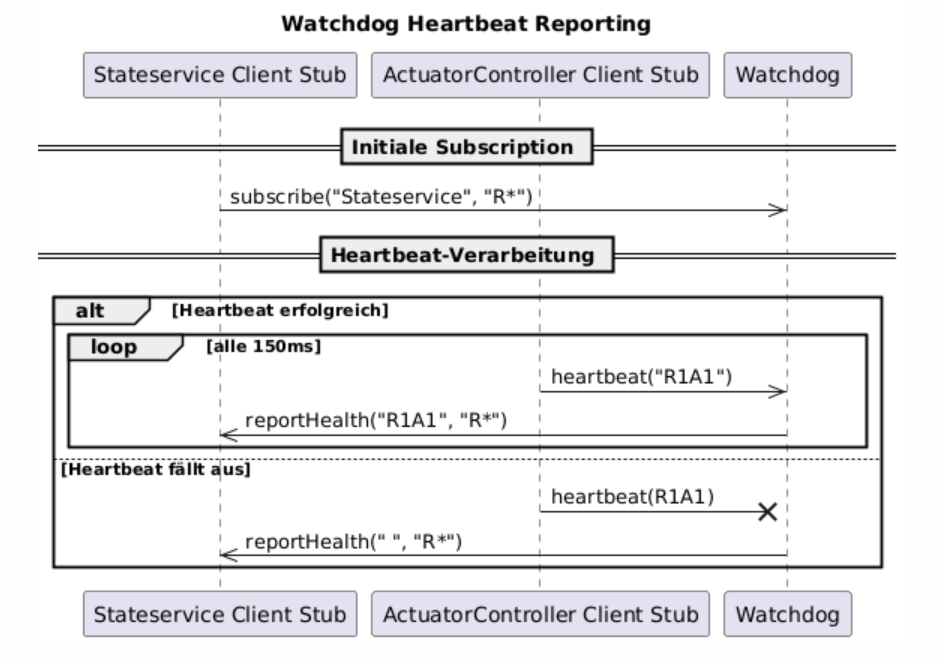
\includegraphics[width=0.8\linewidth]{diagrams/watchdog_16_07.png}
	\caption{Watchdog}
	\label{fig:Watchdog}
\end{figure}






%OLD version, not used anymore i guess !!! 

% \begin{figure}[htbp]
% 	\centering
% 	\includegraphics[width=0.8\textwidth]{diagrams/laufzeitsicht_mit_namensauflösung.png}
% 	\caption{Asynchroner RPC-Anfragedurchlauf inkl. Namensauflösung}
% 	\label{fig:meine-abbildung}
% \end{figure}







\section*{Beschreibung}



